% !TeX spellcheck = cs_CZ
\chapter{Testování}
\label{chap:testovani}
V této kapitole je představeno testování každého z implementovaných útoků a také popis nastavení a infrastruktury laboratorní sítě vytvořené na FEKT VUT.

\section{Schéma zapojení a nastavení testovací sítě}
V laboratoři byly pro testování použity dva fyzické servery pojmenované \textit{DoSgen} (generátor) a \textit{Oběť} jejichž konfigurace je uvedena v tabulce \ref{tab:hw-config-lab}. Na obou serverech je nainstalován operační systém Linux, distribuce Fedora ve verzi 28. Stanice \textit{DoSgen} vystupuje jako generátor útoků, na stanici \textit{Oběť} je nainstalován hypervizor KVM (Kernel-based Virtual Machine). Hypervizor je zde použit jelikož k vykonání požadovaných scénářů jsou požadovány minimálně tři stanice. Konkrétně útočník, amplifikátor a oběť útoku.

\begin{table}[ht]
	\centering
	\caption{Souhrn informací o testovacích stanicích.}
	\label{tab:hw-config-lab}
	\resizebox{\textwidth}{!}{%
		\begin{tabular}{|l|l|l|l|l|l|l|}
			\hline
			Označení        & Model                                                           & OS        & Procesor                                                                              & RAM   & Síťová karta                                                                        & Software \\ \hline
			\textbf{DoSgen} & \begin{tabular}[c]{@{}l@{}}IBM\\ System\\ x3550 M2\end{tabular} & Fedora 28 & \begin{tabular}[c]{@{}l@{}}Intel(R) Xeon(R)\\ L5520,@ 2.27GHz\\ 16 jader\end{tabular} & 32 GB & \begin{tabular}[c]{@{}l@{}}2xNetXtreme\\ II BCM5709\\ Gigabit Ethernet\end{tabular} & DoSgen   \\ \hline
			\textbf{Oběť}   & \begin{tabular}[c]{@{}l@{}}IBM System\\ x3550 M2\end{tabular}   & Fedora 28 & \begin{tabular}[c]{@{}l@{}}Intel(R) Xeon(R)\\ L5520,@ 2.27GHz\\ 16 jader\end{tabular} & 20 GB & \begin{tabular}[c]{@{}l@{}}2xNetXtreme II\\ BCM5709\\ Gigabit Ethernet\end{tabular} & qemu-kvm \\ \hline
		\end{tabular}%
	}
\end{table}

Obě použité fyzické stanice jsou vybaveny dvěma gigabitovými síťovými rozhraními \texttt{enx0} Ethernet. Prvním z nich jsou připojeny do switche, který je připojen do síťě VUT. Pro účely testování byla mezi těmito servery vytvořena izolovaná síť 192.168.2.0/24 do které se stanice připojují svými zbylými síťovými rozhraními. Server DoSgen se do této sítě připojuje pomocí rozhraní \texttt{eth1} a server Oběť skrze \texttt{eth0}.
Názvy těchto rozhraní nekorespondují s reálnými názvy. Toto pojmenování bylo použito z důvodu názornějšího vysvětlení v následující části práce. Celé schéma zapojení je znázorněno na obrázku \ref{fig:vut-lab-schema}. Stanicím v této síti byly přiděleny následující IP adresy:
\begin{itemize}
	\item DoSgen: \textbf{192.168.2.101}/24
	\item Oběť: \textbf{192.168.2.102}/24
\end{itemize}

\begin{figure} [ht]
	\centering
	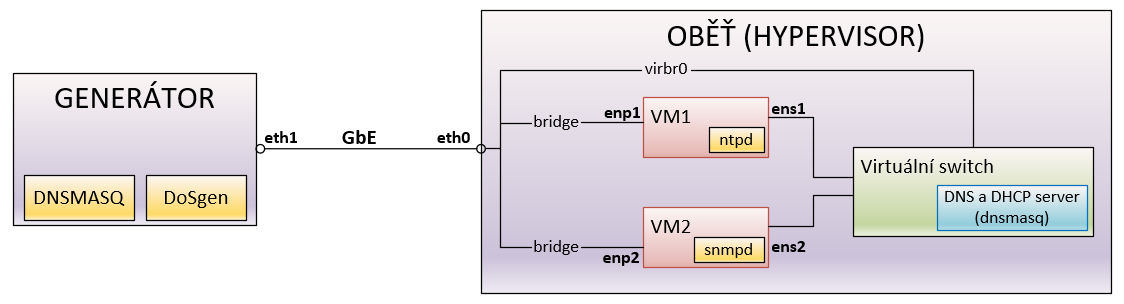
\includegraphics[width=0.9\textwidth]{obrazky/lab_schema.png}
	\caption{Schéma zapojení testovací sítě.}
	\label{fig:vut-lab-schema}
\end{figure}


Stanice vystupující při útoku jako \uv{reflektor} nebo \uv{amplifikátor} a \uv{oběť} jsou plně virtualizované operační systémy skrze hypervizor kernelu (KVM) přistupující ke stejnému síťovému rozhraní \texttt{vnet0}, na něž je připojena i hostitelská stanice. Toto rozhraní je od internetu odděleno prostřednictvím NAT. Pro snazší správu virtualizovaných stanic bylo použito aplikace Virtual Machine Manager ve verzi 1.4.3. V průběhu vývoje a testování jsem využíval nástroje Wireshark pro sledování síťového provozu mezi útočníkem a obětí.

\subsection{Nastavení testovací sítě}
Na hypervizoru bylo použito základní nastavení virtuální sítě. V tomto stavu se virtuální stanice připojují k virtuálnímu switchi v NAT módu. Tento switch je přemostěn přes most \texttt{virbr0} na fyzický síťový adaptér \texttt{eth0}. V této virtuální síti jsou virtuálním stanicím přiřazovány adresy z rozsahu 192.168.122.0/24 programem \texttt{dnsmasq}. Nutno zmínit, že hypervisor má adresu 192.168.122.1. Dále byl pro každou virtuální stanici vytvořen virtuální bridge, který přemosťuje síťová rozhraní \texttt{enp1} a  \texttt{enp2} virtuálních stanic s fyzickým síťovým rozhraním \texttt{eth0} hypervisoru. Takto připojené stanice získávají IP adresy z rozsahu 192.168.2.0/24 a to díky spuštěné službě \texttt{dnsmasq} na serveru DoSgen. Aby bylo možno přistupovat k virtuálním stanicím ze stanice DoSgen, bylo nutné na této stanici do routovací tabulky zapsat statickou cestu do sítě 192.168.122.0/24 přes IP adresu 192.168.2.102.

\subsection{Testování propustnosti sítě}
Tato kapitola se zabývá testováním propustnosti celé sítě a následně zmiňuje výhody a případné nevýhody obou výše zmíněných zapojení.

Na obou fyzických serverech byl spuštěn Apache HTTP server a do jeho kořenového adresáře umístěn binární soubor o velikosti 1 GB. Následně byl z každé stanice tento soubor stažen pomocí programu \texttt{wget}, který zobrazuje rychlost stahování v jednotkách MB/s. Díky této jeho vlastnosti bylo možné změřit propustnost všech spojení v nastavené síti. Data z tohoto testování jsou uvedeny v tabulce \ref{tab:troughput-lab-interfaces}.

\begin{table}[ht]
	\centering
	\caption{Propustnost mezi jednotlivými rozhraními (uvedeno v Mb/s).}
	\label{tab:troughput-lab-interfaces}
	\begin{tabular}{|l|l|l|l|l|}
		\hline
		Rozhraní & eth1 & eth0  & enp1  & ens1  \\ \hline
		eth1     &      & 941   & 525   & 940   \\ \hline
		eth0     & 941  &       & 19200 & 19200 \\ \hline
		enp1     & 525  & 19200 &       & 19200 \\ \hline
		ens1     & 940  & 19200 & 19200 &       \\ \hline
	\end{tabular}
\end{table}

Z těchto dat lze spatřit, že propustnost mezi stanicemi připojenými do virtuálního switche je 2.4 Gb/s a propustnost mezi rozhraními \texttt{eth0} a \texttt{eth1} činí 941 Mb/s. Pokud však generujeme útok ze stanice DoSgen a cílíme jej na virtuální stanici skrze virtuální switch, bude maximální propustnost limitována propustností mezi rozhraními \texttt{eth0} a \texttt{eth1}.
Při využití přemostěného spojení skrze rozhraní \texttt{enp1} a \texttt{enp2} bylo dosaženo maximální propustnosti 525 Mb/s. Jelikož předchozí uvedené zapojení dosáhlo vyšší propustnosti, byly tyto spojení spolu se síťovými rozhraními odstraněny a při testování útoků nebyly využity.

%instalace netdata
%testovani probiha z prikazoveho radku, popsat proc


\subsection{Použitý software} %strucne ke kazdemu co, k cemu, proc jsem zvolil, licence
Pro monitorování využití CPU, paměti RAM, síťových rozhraní a jiných veličin byl použit program Netdata. Tento program běží jako démon na stanici, na které chceme statistická data sbírat. Netdata získaná data ukládá do databáze, při prohlížení je tedy možno vracet se i v čase a prohlížet historická data.

\section{Testování útoku NTP Flood}
Operační systém, na kterém je spuštěn NTP sever, jsem musel zvolit Fedora 14, jehož datum vydání bylo 2.\ 11.\ 2010. Bylo nutno zvolit takto starou verzi z důvodu opravy chyby v balíčku \texttt{ntp} v pozdějších vydáních. Nainstalován byl tedy balíček \texttt{ntp-4.2.6p3}. Na tomto stroji musel být správně nakonfigurován firewall tak, abych byl schopen službu NTP kontaktovat z jiné stanice. Následně byl změněn konfigurační soubor pro NTP server způsobem popsaným v kapitole \ref{subsec:ntp_flood}.

Na serveru, který slouží jako oběť tohoto útoku je spuštěn operační systém Fedora 28 Server a nainstalován Apache server ve verzi \texttt{httpd-2.4.29}. Firewall je také patřičně nakonfigurován.

Dalším krokem je vygenerování falešných uživatelů dotazujících se na NTP server. To provedeme spuštěním skriptu a následně si můžeme ověřit pomocí příkazu \texttt{ntpdc}, že záznamů je požadované množství. Pro spuštění těchto příkazů je nutno mít nainstalované balíčky \texttt{ntp} v libovolné verzi a \texttt{python3-scapy}.

\begin{lstlisting}[language=bash]
python3 fake_ntp_hosts.py
ntpdc -n -c monlist 192.168.124.14 | wc -l
\end{lstlisting}

\newpage

\noindent V tomto okamžiku nic nebrání spuštění útoku a to následovně:
\begin{lstlisting}
./dosgen -i virbr0 -P 4 --ntp -s 192.168.124.129 \
	-d 192.168.124.14
\end{lstlisting}

Nyní je NTP server zahlcován dotazy. Odpověďi na ně zasílá na IP adresu oběti. Výstup aplikace DoSgen lze vidět na obrázku \ref{fig:dosgen_run_ntp-img}

\begin{figure} [ht]
	\centering
	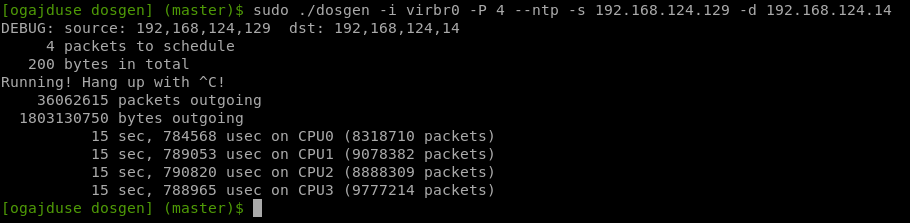
\includegraphics[width=0.9\textwidth]{obrazky/dosgen_terminal_run_ntp.png}
	\caption{Spuštění aplikace DoSgen se zvoleným NTP útokem.}
	\label{fig:dosgen_run_ntp-img}
\end{figure}

Při sledování provozu v programu Wireshark můžeme vidět, že na NTP server je vyslán požadavek \uv{monlist} a NTP server na něj odpovídá, přičemž zamění zdrojovou adresu zamění za cílovou a naopak a paket je tak vyslán na server oběti, která o něj nejeví zájem, tudíž na každý z nich odpovídá ICMP zprávou typu 3 s kódem 9 (Host administratively prohibited).

\begin{figure} [h]
	\centering
	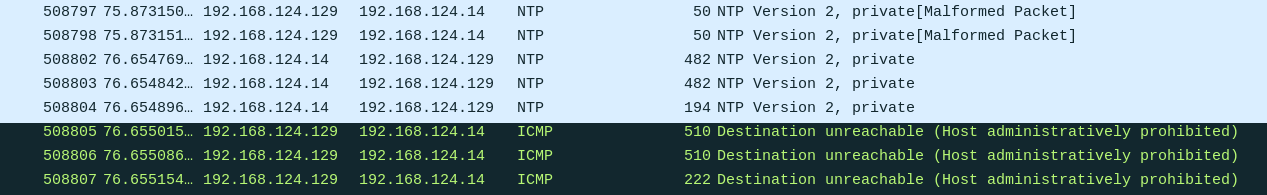
\includegraphics[width=0.9\textwidth]
	{obrazky/mon_getlist_1_wireshark_with_icmp_and_reply.png}
	\caption{Průběh NTP útoku zobrazený v  aplikaci Wireshark.}
	\label{fig:mon_getlist_1_wireshark_with_icmp_and_reply-img}
\end{figure}

Celá tato komunikace je zachycena na obr. \ref{fig:mon_getlist_1_wireshark_with_icmp_and_reply-img}. Pakety s číslem 508797 a 508798 jsou vygenerované nástrojem DoSgen. Následující tři pakety, tedy pakety s číslem 508802-508804 jsou odpovědí NTP serveru. Tato odpověď obsahuje pouze 13 hostů, v případě, že nám server vrátí 600 hostů, odpověď od serveru bude mnohonásobně větší.

Trafgen dokáže v případě konfigurace NTP paketu generovat provoz o velikosti 300 Mb/s. Tento fakt není na škodu, jelikož trafgen generuje stále větší počet požadavků, než je jeden NTP server schopen obsloužit. Vezměme na vědomí, že nejstěžejnějším bodem při realizaci tohoto útoku je samotný NTP server, na kterém záleží, jak velkým objemem dat bude stanice oběti zahlcena. Jeden NTP server je schopen vygenerovat provoz o velikosti 100 Mb/s.

Na základě toho byl při testování použit větší počet NTP serverů, zahlcující jedinou oběť a spuštěn stejný počet instancí DoSgenu. Každá instance generovala provoz za použití jednoho jádra.

Testovací scénář započal s počtem 5 NTP serverů. V tomto případě NTP servery dokázaly vygenerovat provoz o velikosti 219 Mb/s. Po celou dobu útoku byl na systému oběti zvýšené procentuální využití CPU. Toto chování je znázorněno na obrázcích \ref{fig:graph_ntp_traffic_5ampl} a \ref{fig:graph_cpu_traffic_5ampl}.


\begin{figure} [h]
	\centering
	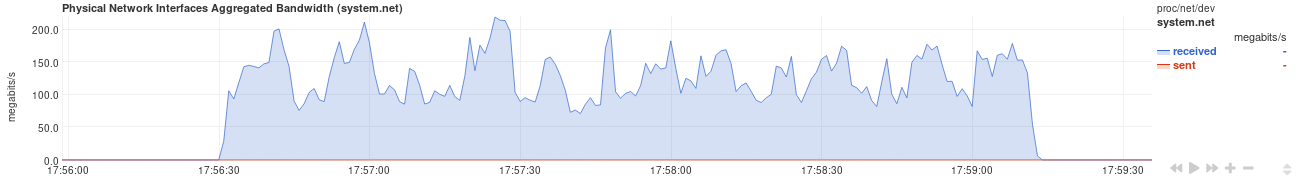
\includegraphics[width=0.9\textwidth]
	{obrazky/grafy/graph_ntp_traffic_5ampl.png}
	\caption{Průběh NTP útoku s 5 NTP servery, síťový provoz na straně oběti.}
	\label{fig:graph_ntp_traffic_5ampl}
\end{figure}

\begin{figure} [h]
	\centering
	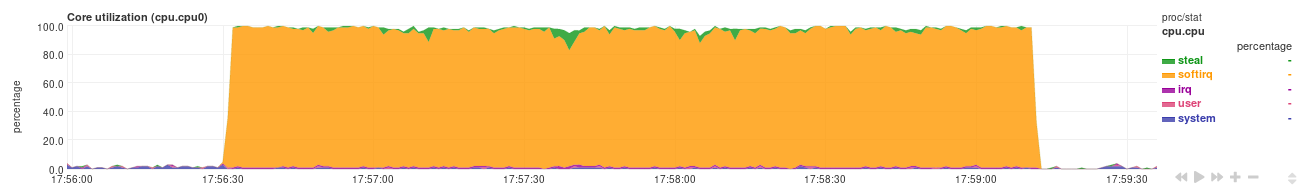
\includegraphics[width=0.9\textwidth]
	{obrazky/grafy/graph_ntp_cpu_5ampl.png}
	\caption{Průběh NTP útoku s 5 NTP servery, zatížení CPU na straně oběti.}
	\label{fig:graph_cpu_traffic_5ampl}
\end{figure}

Následoval scénář se 6 NTP servery. V tomto případě zde došlo k anomálii, jelikož při zahlcení oběti provozem ze 6 NTP serverů je předpoklad, že vygenerovaný provoz bude vyšší, než u předchozího scénáře. Tak se však nestalo a špička tohoto scénáře je na úrovni 160 Mb/s.
Tuto situaci přibližuje graf \ref{fig:graph_ntp_traffic_5ampl_vs6ampl}.

\begin{figure} [h]
	\centering
	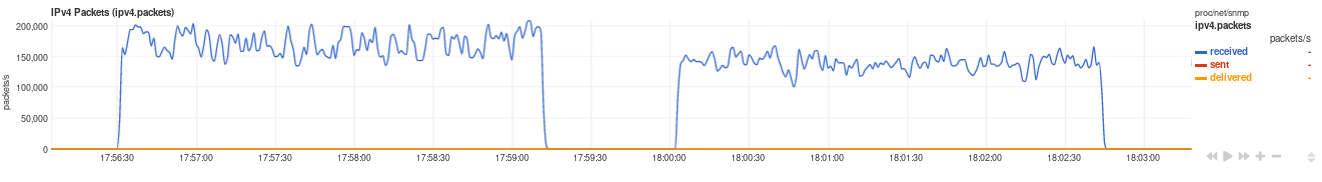
\includegraphics[width=0.9\textwidth]
	{obrazky/grafy/graph_ntp_traffic_5ampl_vs6ampl.png}
	\caption{Porovnání průběhu NTP útoku s 5 a 6 NTP servery, síťový provoz na straně oběti.}
	\label{fig:graph_ntp_traffic_5ampl_vs6ampl}
\end{figure}

Toto chování připisuji virtuálnímu switchi, který se choval nestandardně i při útoku za použití jednoho NTP serveru. Toto chování spočívalo ve zvýšené odezvě při komunikaci mezi klienty ve stejné síti, přičemž tito klienti neparticipovali na útoku.

Testování tohoto útoku je vhodnější na fyzické infrastruktuře, která se dá lépe konfigurovat a poskytne vyšší výkon než poskytuje virtuální switch hypervizoru.

\section{Testování útoku SNMP Flood}
Testování tohoto útoku mělo velmi stejný průběh jako testování útoku předešlého. Tedy bylo vytvořeno 8 virtuálních stanic se stejnou konfigurací. Tyto stanice vystupovaly v síti jako SNMP agenti. Útočník, DoSgen, na ně zasílal dotazy s podvrženou IP adresou. Tento provoz byl agentem amplifikován a zasílán na stanici oběti. Agenti byli nakonfigurováni dle postupu uvedeného v kapitole \ref{subsec:snmp_flood_impl}.

U tohoto scénáře byla zaznamenána stejná anomálie, jako ve scénáři s protokolem NTP. Největší objem dat zaslaný agenty v jednu chvíli byl za použití 7 agentů. Zatížení procesoru oběti je znázorněno na obrázku \ref{fig:graph_snmp_cpu_5ampl} a počet paketů přijatých na síťovém rozhraní oběti v Mb/s na obrázku \ref{fig:graph_snmp_traffic_5ampl}.

\begin{figure} [h]
	\centering
	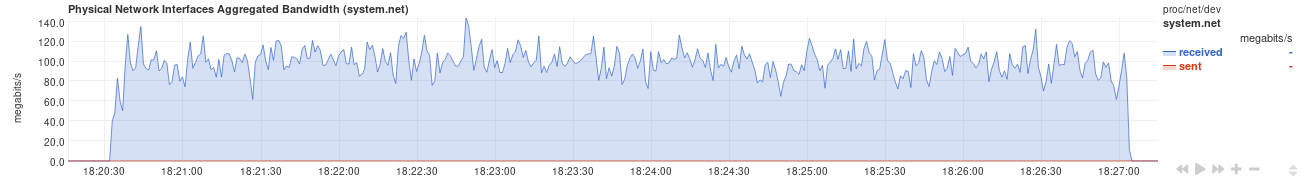
\includegraphics[width=0.9\textwidth]
	{obrazky/grafy/graph_ntp_traffic_7ampl.png}
	\caption{Průběh SNMP útoku se 7 SNMP agenty, síťový provoz na straně oběti.}
	\label{fig:graph_snmp_traffic_5ampl}
\end{figure}

\begin{figure} [h]
	\centering
	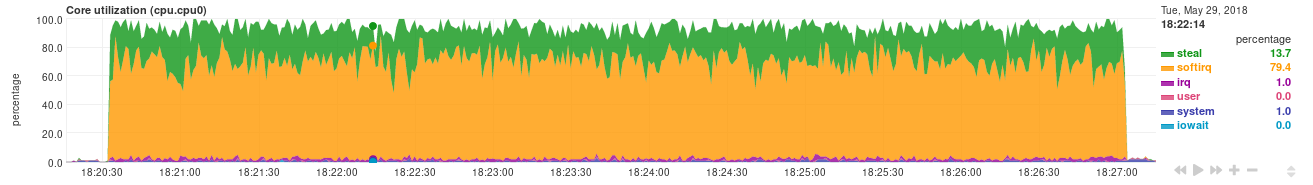
\includegraphics[width=0.9\textwidth]
	{obrazky/grafy/graph_ntp_cpu_7ampl.png}
	\caption{Průběh SNMP útoku se 7 SNMP agenty, zatížení CPU na straně oběti.}
	\label{fig:graph_snmp_cpu_5ampl}
\end{figure}



\section{Testování útoku SSDP Flood}
Tento útok byl testován  stejným způsobem jako předchozí dva útoky. V testovací síti bylo přítomno 5 UPnP zařízení, jedna oběť a generátor.

V tomto případě byla síť zahlcena natolik, že žádná ze stanic v síti nebyla schopna kontaktovat jinou stanici v síti. Z obrázku \ref{fig:ping_ntp_5_ampl} je tato situace zřejmá. První 4 odpovědi na ICMP echo byly úspěšné s časem pod 0 ms. Čtvrtá odpověď od stanice 192.168.122.210 byla doručena v čase, kdy útok započal. Odpověď na následné dotazy již nebyly stanici, která zasílala ICMP echo doručeny. 

\begin{figure} [h]
	\centering
	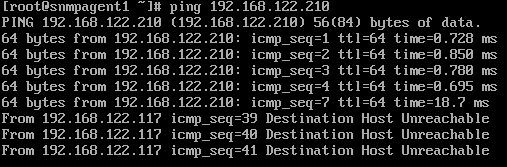
\includegraphics[width=0.9\textwidth]
	{obrazky/grafy/ping_ntp_5ampl.png}
	\caption{Test odezvy stanice v síti, ICMP ping.}
	\label{fig:ping_ntp_5_ampl}
\end{figure}
